\chapter{The Translating Coil Fluxmeter}
The fluxmeter consists of several components. A PCB with
printed flux pickup coils, fast digital integrators, a rotary
encoder and a laser tracker system for geometric positioning measurements.

\begin{figure}[!h]
    \centering
    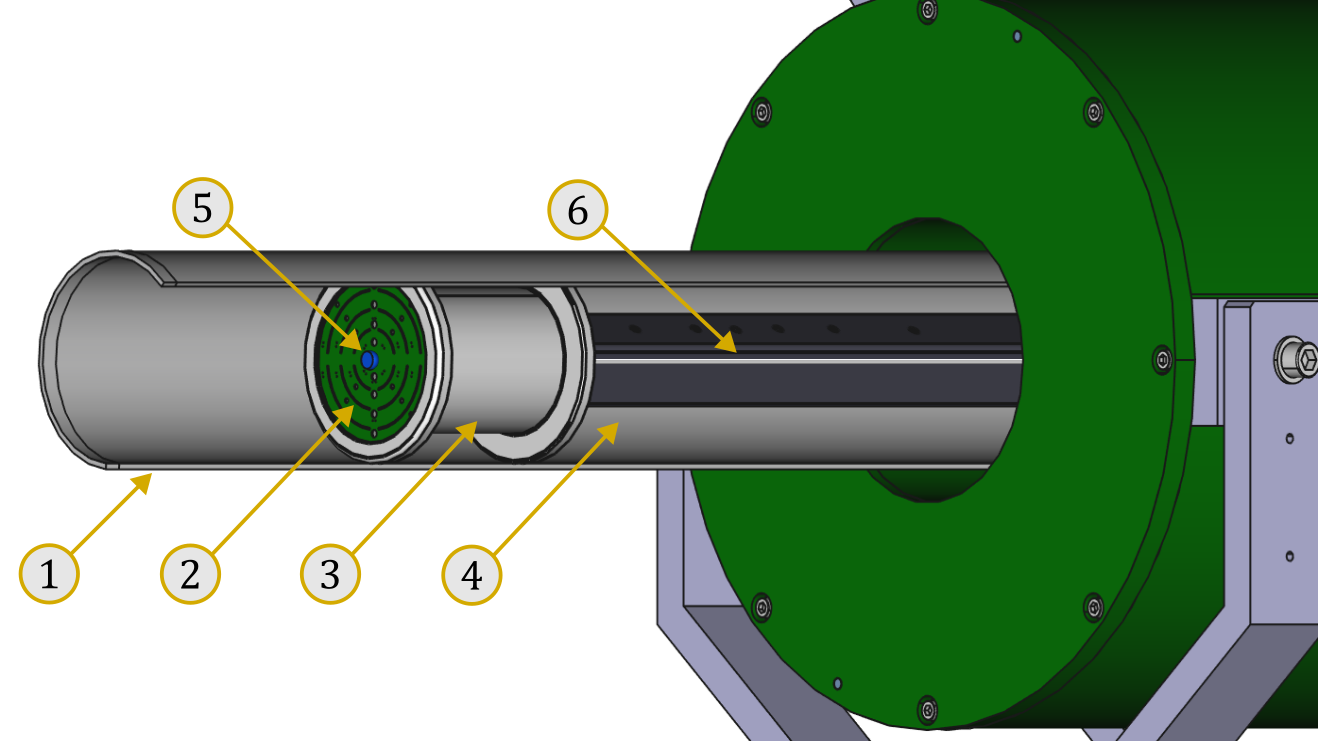
\includegraphics[width=0.7\textwidth]{figs/elena}
    \caption{The fluxmeter assembly going through a solenoid magnet. \\
        1. Guiding Tube, 2. Fluxmeter PCB, 3. PCB Sledge, 4. Supporting arm,
        5. Laser Reflector, 6. Encoder Wire.}
    \label{fig:elena}
\end{figure}

To move the PCB through the magnet aperture, a support assembly was made as
seen in figure \ref{fig:elena}. The coil cables are run through the supporting
arm, which is also used to push and pull the fluxmeter through the tube. A
wire is connected to the PCB sledge on one end, and spooled up around
a rotating encoder on the other end. In the middle of the PCB, a
reflector is mounted for the laser tracker.

\section{PCB printed coils}
The coil PCB has 21 different coils.
These coils are in the shapes of disks or annulus segments.
A render of the pcb can be seen in figure
\ref{fig:pcb}. The disks are denoted $D_l$ and the
annulus segments by $Q_{q, l}$ where $l$ is the radial layer and
$q$ is the quadrant, as seen in figure \ref{fig:nomenclature}.

\begin{figure}[!h]
    \centering
    \begin{subfigure}[b]{0.5\linewidth}
        \centering
        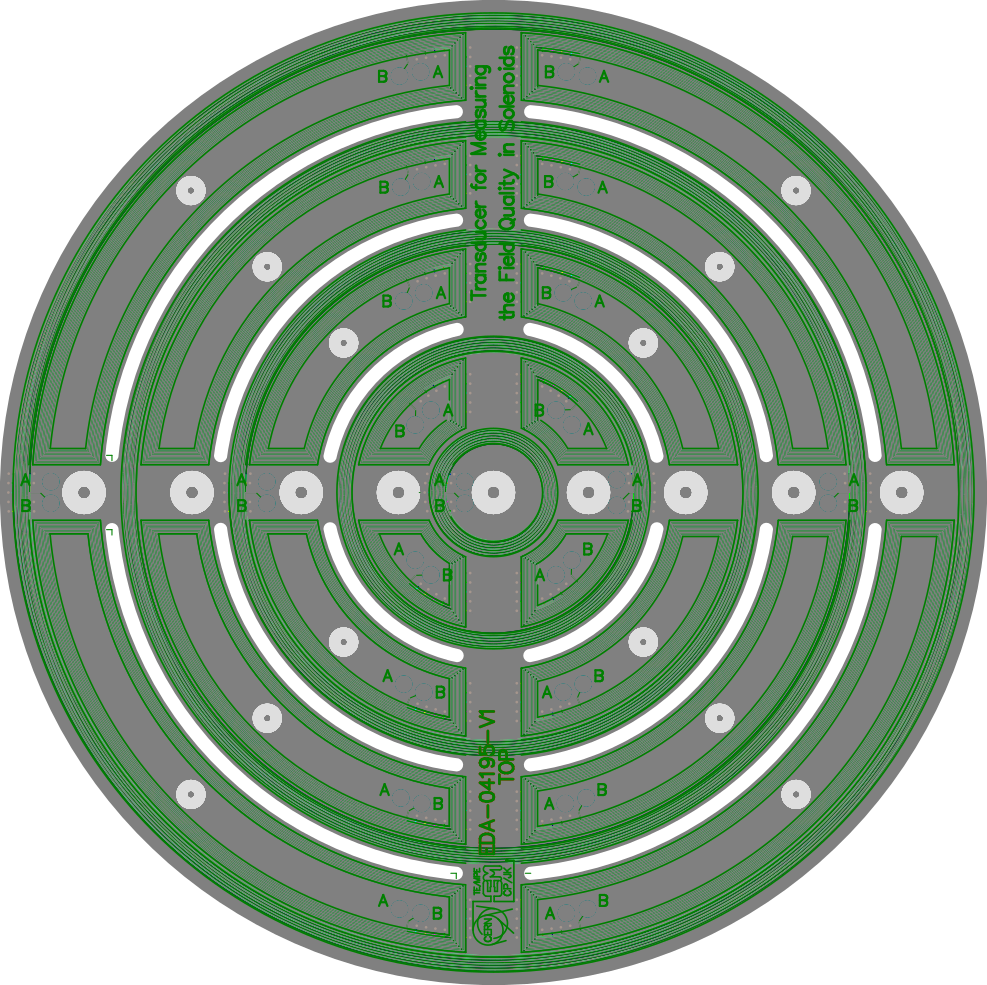
\includegraphics[width=0.8\linewidth]{figs/pcb}
        \caption{The fluxmeter PCB.}
        \label{fig:pcb}
    \end{subfigure}
    \hfill
    \begin{subfigure}[b]{0.4\linewidth}
        \centering
        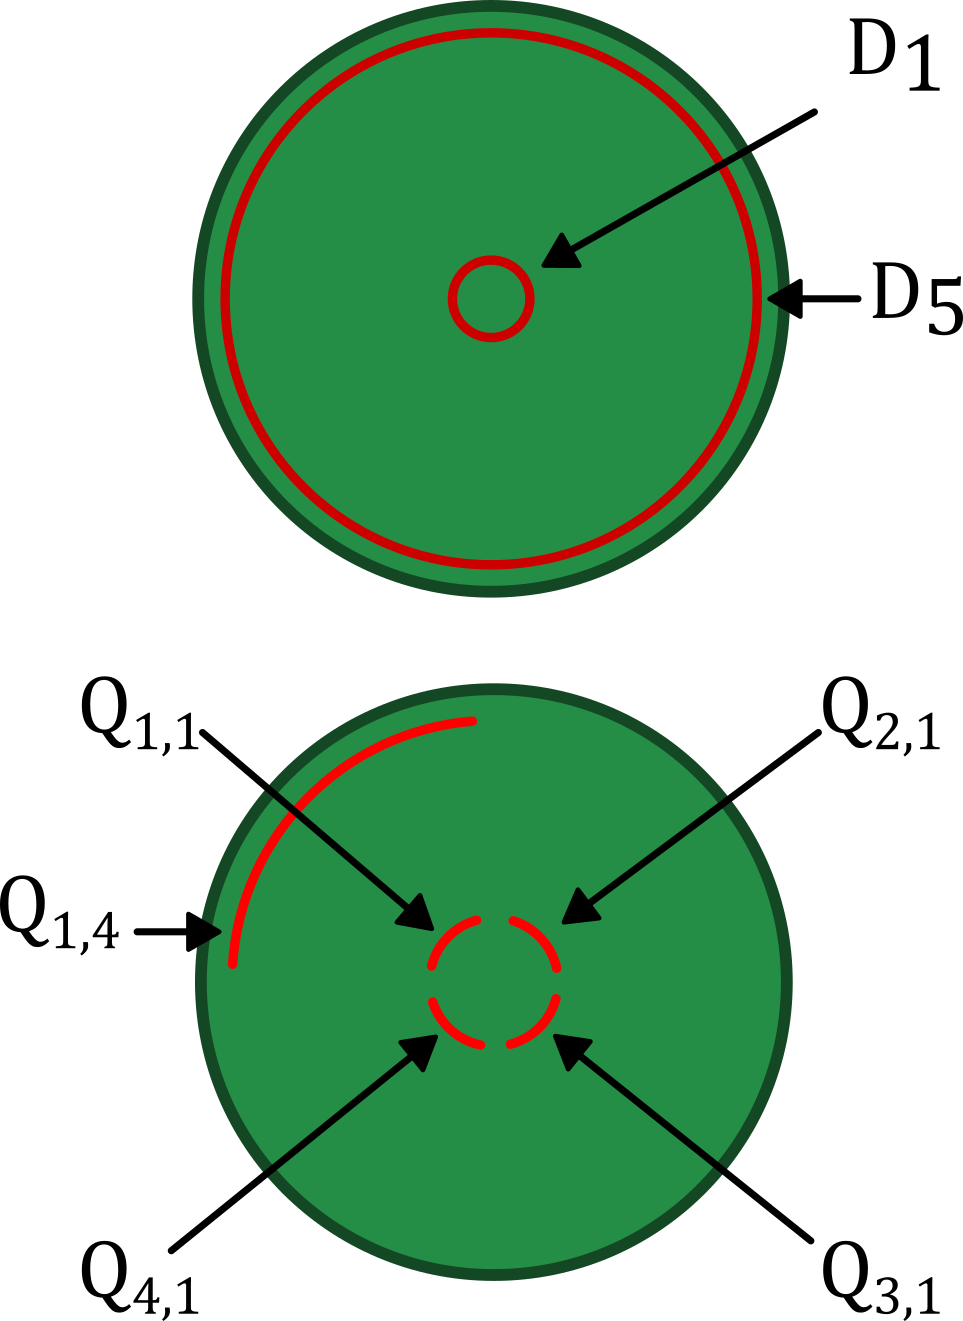
\includegraphics[width=0.8\linewidth]{figs/nomenclature.png}
        \caption{Nomenclature of the PCB coils.}
        \label{fig:nomenclature}
    \end{subfigure}
    \caption{}
\end{figure}

During measurements, the magnet is magnetized with a constant current.
As the coils move through the magnet, a voltage is induced according
to Faradays Law, equation \ref{eq:faraday}. Although the field is
static, since the fluxmeter is moving it will still see a delta
flux with respect to time.

\section{The Measurement Assembly}
A picture of the magnet with the guiding tube and tube clamps can be seen in
figure \ref{fig:magnetassembly}. In figure \ref{fig:leica}, the laser tracker
can be seen, locked onto the target on the fluxmeter pcb.

\begin{figure}[!h]
    \centering
    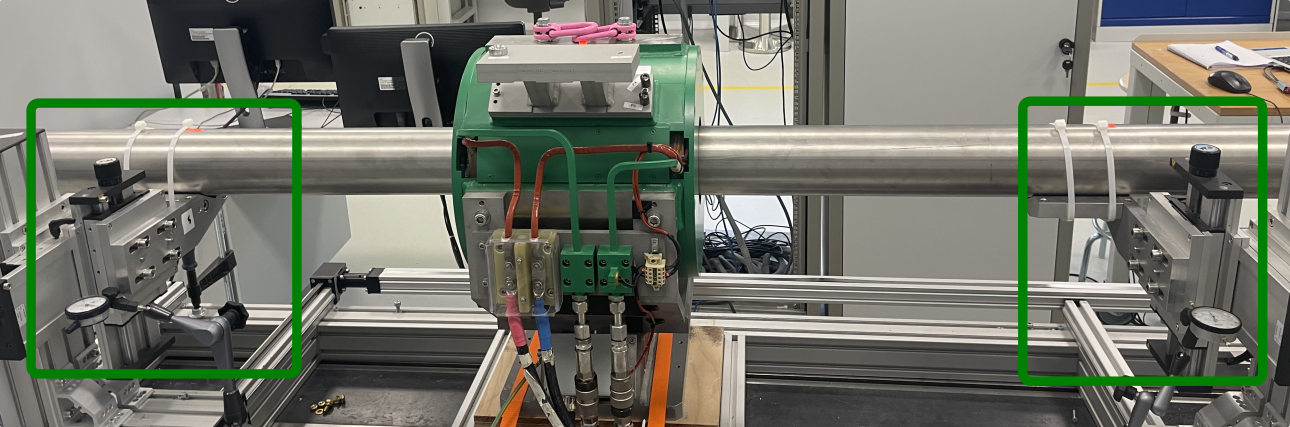
\includegraphics[width=0.7\textwidth]{figs/magnet-assembly}
    \caption{Guiding tube in the magnet. Tube clambs marked in green rectangles.}
    \label{fig:magnetassembly}
\end{figure}

\begin{figure}[!h]
    \centering
    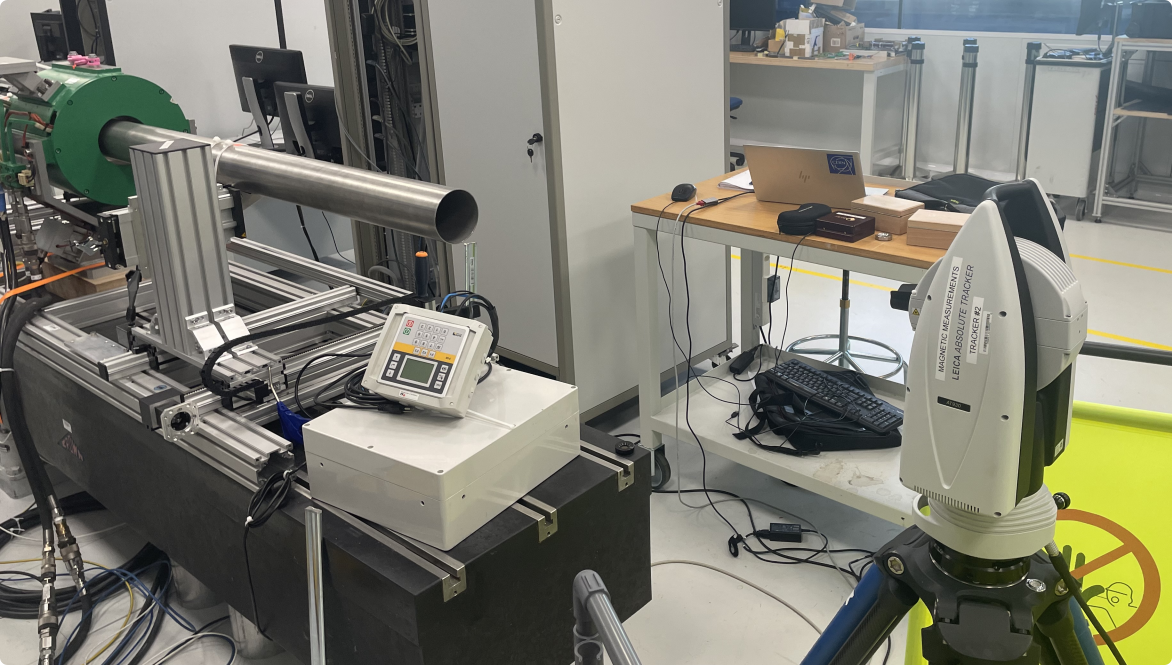
\includegraphics[width=0.7\textwidth]{figs/leica}
    \caption{Laser tracker, looking into the guiding tube.}
    \label{fig:leica}
\end{figure}

\section{Geometric Measurements}
The laser tracker works by shooting a laser at a reflector, and then
measuring the time of flight. The accuracy depends on the reflector
type and measurement time, but an upper limit of
0.2 mm is a reasonable estimate according to the
specifications of both the reflectors and laser tracker
used. \cite{leica_manual}.

Firstly, scans were done of a network of reflectors around the
room. These points were then used as a baseline to locate the
laser tracker at the start of each measurement campaign, or when
the laser tracker needed to be moved. A cluster of points were
taken of the magnet itself. These points
were then fitted to a cylinder. Using a 3D model of the
solenoid, a coordinate system could be constructed
with its origin at the geometric center of the magnet.
The $z$ axis was chosen as the solenoidal axis, pointing
in the field direction. $y$ was chosen as the axis
pointing up, opposite to gravity, leaving $x$ as 
the axis parallel to the ground.

Furthermore, two planes were constructed at the positions
of the clamps holding the fluxmeter guiding tube. The
positions of these clamps could accurately be moved in
both lateral dimensions using precision dials. In effect,
the tube has two anchor points that can be moved along
the aforementioned planes, so that it can be aligned (or misaligned)
as desired.

\begin{figure}[!h]
    \centering
    \includegraphics[width=0.7\textwidth]{figs/3Dscan}
    \caption{3D scans of the measurement assembly.
        1: Laser Tracker, 2: 3D scan of the solenoid,
        3: Network Point, 4: Tube clamp positioning planes.
        3D scans fitted using Spatial Analyzer \cite{spatial_analyzer}.}
    \label{fig:3dscan}
\end{figure}

\section{Positional Encoder}
The positional encoder is a rotating encoder connected to a wire spool.
As the fluxmeter moves through the the magnet, it pulls on the wire,
spinning the rotating encoder. The encoder is of a 16 bit type, meaning
it sends out a pulse $2^{16} = 65536$ times per turn. These pulses were
decimated by a factor of 32, giving 2048 pulses per turn. By triggering
the laser tracker with these pulses, it was found that one turn corresponds
to a fluxmeter translation of $23.0095$ cm along the axis. The distance
per pulse were measured to be $0.11$ mm, with a standard deviation of
$6.69 \, \mu \text{m}$.

\begin{figure}[h]
    \centering
    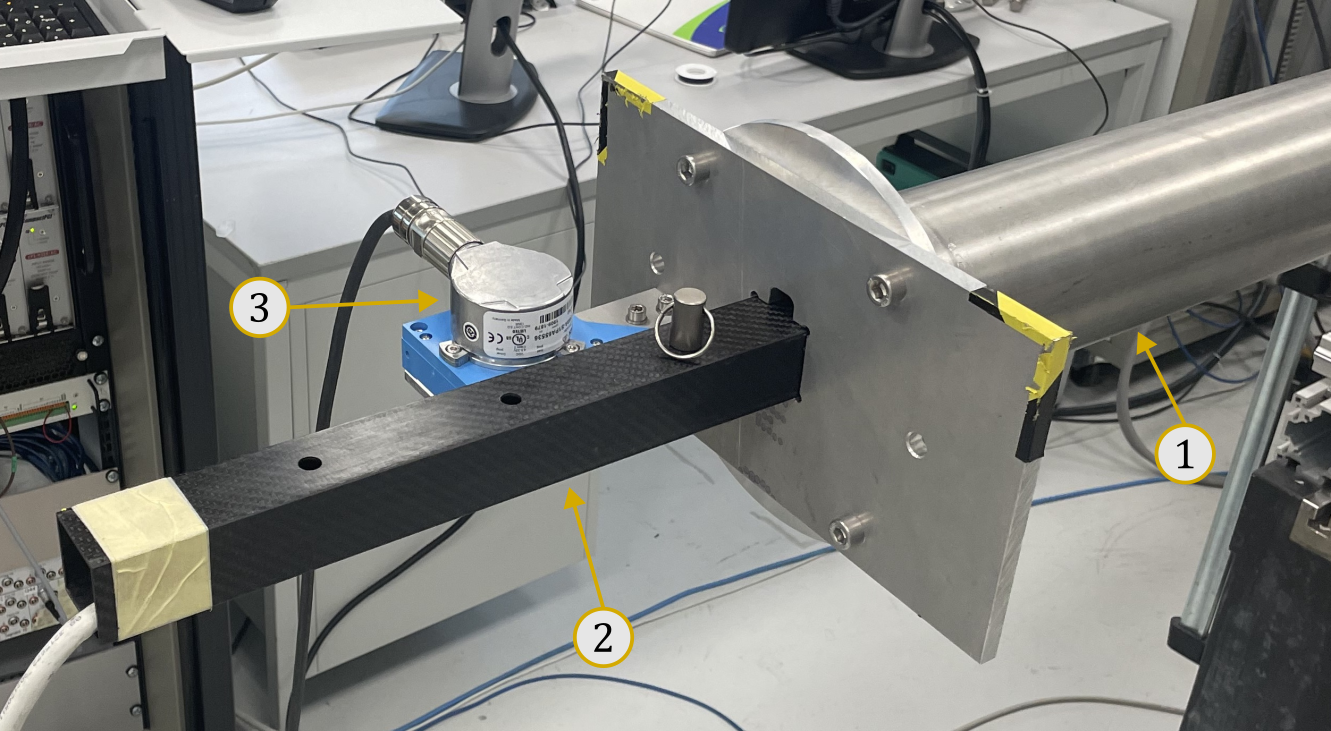
\includegraphics[width=0.7\textwidth]{figs/encoder}
    \caption{One end of the fluxmeter guiding tube (1), with guiding arm (2)
        and positional encoder (3).}
    \label{fig:encoderpic}
\end{figure}

\section{Fast Digital Integrators}
The fast digital integrators (FDI:s) are used to align flux measurements
with their geometric positions. They continuously sample the voltages
from the fluxmeter coils at $500$ kHz. For every trigger from the encoder,
the FDI:s outputs the integrated voltage with respect to time, with the
integration limits being the last two triggers. This
corresponds to the change in flux between two trigger times $t_i$. Since these
triggers are fired at specific points along the fluxmeter axis, the
delta fluxes can easily be mapped from time to geometric position, as in
equation \ref{eq:deltaPhi}.

\begin{equation}
    \Delta \Phi_i =
    \int \limits_{t_{i-1}}^{t_i} \frac{d}{dt}\Phi dt
    = \Phi_{z_{i-1}} - \Phi_{z_{i}} = \Delta \Phi[z_i]
    \label{eq:deltaPhi}
\end{equation}

The flux through a coil for each $z$ position is then easily obtained
by taking the cumulative sum of the delta fluxes, as in equation
\ref{eq:Phiz}.

\begin{equation}
    \Phi[z_i] = \sum \limits_{k=0}^i \Delta \Phi[z_i]
    \label{eq:Phiz}
\end{equation}

The advantage of this approach is that the measurements are invariant
to the speed at which the fluxmeter moves through the magnet, within limits.
The lower limit on the translating speed is such that the induced
voltage in the coils is higher than the noise floor.
The upper limit is decided by the sampling frequency of the FDI:s.
As long as a sufficient number of voltage samples are gathered between
each encoder trigger, the measurements are repeatable to a high accuracy.

Furthermore, the integration operation of the FDI:s act as a
low pass filter, removing high frequency noise in the voltage
signals.

As seen in figure \ref{fig:measurement-assembly}, the encoder triggers
both the FDI:s and the laser tracker, giving accurate positions coupled
to the delta fluxes. This way, the geometric repeatability of the 
measurements were substantially increased, since the laser tracker 
had fixed coordinate frame in relation to the network points.

\tikzset{sensor/.style={rectangle, rounded corners, minimum width=3cm, minimum height=1cm,text centered, draw=black, fill=green!30}}
\tikzset{process/.style={rectangle, minimum width=3cm, minimum height=1cm, text centered, draw=black, fill=orange!30}}
\tikzset{output/.style={diamond, minimum width=3cm, minimum height=1cm, text centered, draw=black, fill=white!30}}

\begin{figure}[h]
    \centering
    \begin{tikzpicture}[node distance=3cm]
        \node (coils) [sensor, align=center] {Fluxmeter\\PCB};
        \node (encoder) [sensor, below of=coils] {Encoder};
        \node (triggers) [right of=encoder] {Triggers};

        \node(leica) [process, right of=triggers, align=center]
        {Laser\\Tracker};

        \node(FDI) [process, right of=coils, xshift=3cm]
        {FDI:s};

        \node(output) [output, right of=FDI, yshift=-1.5cm] {Output};
        \coordinate [below of=FDI, yshift=1.5cm] (bFDI);

        \draw [->] (coils) -- node[anchor=south]{Voltages}(FDI);
        \draw [->] (FDI) -| node[anchor=south]{$\Delta$ Fluxes} (output);
        \draw [->] (encoder) -- (triggers);
        \draw [->] (triggers) -- (leica);
        \draw [->] (triggers) |- (bFDI) -- (FDI);
        \draw [->] (leica) -| node[anchor=north]{Positions} (output);
    \end{tikzpicture}
    \caption{Flowchart for the measurement assembly.}
    \label{fig:measurement-assembly}
\end{figure}